\chapter{Generating Series}

Generating series are the main tool of the enumeration half of the course. The idea is to
package an entire sequence of counting numbers $a_0, a_1, a_2, \dots$ into one algebraic
object $\sum a_n x^n$, and then to translate set constructions (disjoint unions, Cartesian
products, sequences) into algebra (sums, products, inverses).

\section{Weight functions and generating series}

\begin{definition}[Weight function]
Let $S$ be a set. A \emph{weight function} on $S$ is a function $w : S \to \Z_{\ge 0}$ such
that for every $n$, the set $\{\sigma \in S : w(\sigma) = n\}$ is finite.
\end{definition}

\begin{definition}[Generating series]
The \emph{generating series} of $S$ with respect to $w$ is
\[
\Phi_S(x) = \sum_{\sigma \in S} x^{w(\sigma)} = \sum_{n \ge 0} a_n x^n,
\qquad a_n = \abs{\{\sigma \in S : w(\sigma) = n\}}.
\]
\end{definition}

So the coefficient of $x^n$ is the number of objects of weight $n$. We write $\coef{n}A(x)$
for the coefficient of $x^n$ in $A(x)$.

\begin{example}
Let $S$ be the set of all subsets of $[n]$ with $w(T) = \abs{T}$. Then
$\Phi_S(x) = \sum_{k} \binom{n}{k} x^k = (1+x)^n$.
\end{example}

\begin{example}
Let $S$ be the set of outcomes of rolling two (distinguishable) six-sided dice, with weight the
total. Then $\Phi_S(x) = (x + x^2 + \cdots + x^6)^2$, and
$\coef{7}\Phi_S(x) = 6$: there are six ways to roll a total of $7$.
\end{example}

Laying out the $36$ outcomes in a grid, the outcomes of a given weight lie on an anti-diagonal;
the shaded one has the six outcomes of total $7$:
\begin{center}
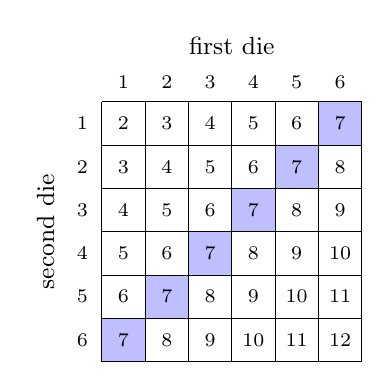
\begin{tikzpicture}[scale=0.55]
  \foreach \i in {1,...,6} { \foreach \j in {1,...,6} {
    \pgfmathtruncatemacro{\s}{\i+\j}
    \ifnum\s=7 \fill[blue!25] (\i-1,6-\j) rectangle (\i,7-\j); \fi
    \node[font=\scriptsize] at (\i-0.5,6.5-\j) {\s};
  } }
  \draw (0,0) grid (6,6);
  \foreach \i in {1,...,6} {
    \node[font=\scriptsize] at (\i-0.5,6.45) {\i};
    \node[font=\scriptsize] at (-0.45,6.5-\i) {\i};
  }
  \node[font=\small] at (3,7.3) {first die};
  \node[font=\small,rotate=90] at (-1.3,3) {second die};
\end{tikzpicture}
\end{center}

Two simple facts are worth knowing: $\Phi_S(1) = \abs{S}$ when $S$ is finite, and
$\Phi_S'(1) = \sum_{\sigma \in S} w(\sigma)$, so the average weight is $\Phi_S'(1)/\Phi_S(1)$.
For subsets of $[n]$: $\frac{n(1+1)^{n-1}}{2^n} = \frac{n}{2}$, as expected.

\section{Formal power series}

\begin{definition}[Formal power series]
A \emph{formal power series} is an expression $A(x) = \sum_{n \ge 0} a_n x^n$ with
coefficients $a_n \in \Q$ (or $\R$, $\C$). Two series are equal iff all their coefficients
are equal. Sum and product are defined by
\[
A(x) + B(x) = \sum_{n \ge 0}(a_n + b_n) x^n, \qquad
A(x)B(x) = \sum_{n \ge 0}\Big(\sum_{k=0}^n a_k b_{n-k}\Big) x^n.
\]
\end{definition}

The word \emph{formal} means we never substitute a number for $x$ and never worry about
convergence; $x$ is just a placeholder that keeps track of indices. Every coefficient of a sum
or product is a \emph{finite} computation, so these operations are always defined.

\begin{definition}[Inverse]
$B(x)$ is an \emph{inverse} of $A(x)$ if $A(x)B(x) = 1$. We write $B(x) = A(x)^{-1} = 1/A(x)$.
\end{definition}

\begin{theorem}
A formal power series $A(x) = \sum a_n x^n$ has an inverse if and only if $a_0 \ne 0$. The
inverse is unique when it exists.
\end{theorem}
\begin{proof}
If $AB = 1$ then comparing constant terms, $a_0 b_0 = 1$, so $a_0 \ne 0$. Conversely suppose
$a_0 \neq 0$. We need $b_0, b_1, \dots$ with $a_0 b_0 = 1$ and
$\sum_{k=0}^n a_k b_{n-k} = 0$ for $n \ge 1$. Set $b_0 = 1/a_0$ and, recursively,
\[
b_n = -\frac{1}{a_0}\sum_{k=1}^{n} a_k b_{n-k} \qquad (n\ge 1).
\]
These equations determine each $b_n$ uniquely from the earlier ones, so the inverse exists and
is unique.
\end{proof}

\begin{example}[Geometric series]
$(1-x)(1 + x + x^2 + \cdots) = 1$, since the coefficient of $x^n$ on the left is $1 - 1 = 0$ for
$n \ge 1$. So $\frac{1}{1-x} = \sum_{n \ge 0} x^n$. Replacing $x$ by $cx$,
$\frac{1}{1-cx} = \sum_{n\ge0} c^n x^n$, and also $\frac{1 - x^{m+1}}{1-x} = 1 + x + \cdots + x^m$.
\end{example}

\begin{definition}[Composition]
If $B(x)$ has constant term $0$ then $A(B(x)) = \sum_n a_n B(x)^n$ is a well-defined formal
power series, because $B(x)^n$ only involves powers $x^n$ and higher, so each coefficient of
$A(B(x))$ is a finite sum.
\end{definition}

For example $\frac{1}{1 - (x + x^2)}$ is $A(B(x))$ with $A(y) = \frac{1}{1-y}$ and
$B(x) = x + x^2$. But $\sum_n (1+x)^n$ is \emph{not} defined: its constant term would be
$1 + 1 + 1 + \cdots$.

\begin{theorem}[Negative binomial theorem]
For an integer $k \ge 1$,
\[
\frac{1}{(1-x)^k} = \sum_{n \ge 0} \binom{n+k-1}{k-1} x^n.
\]
\end{theorem}
\begin{proof}
$\frac{1}{(1-x)^k} = \left(\sum_{m \ge 0} x^m\right)^k$, so the coefficient of $x^n$ is the
number of $k$-tuples $(m_1,\dots,m_k)$ of non-negative integers with sum $n$, which is the
number of multisets of size $n$ with $k$ types, namely $\binom{n+k-1}{k-1}$.
\end{proof}

\begin{important}[Pitfall: shifting]
When extracting coefficients, keep track of shifts: $\coef{n}\, x^k A(x) = \coef{n-k} A(x)$,
which is $0$ if $n < k$. For example $\coef{n} \frac{x^3}{(1-x)^2} = \binom{n-3+1}{1} = n-2$
for $n \ge 3$ and $0$ otherwise.
\end{important}

\section{The sum and product lemmas}

\begin{lemma}[Sum lemma]
Let $A$ and $B$ be disjoint sets and $w$ a weight function on $A \cup B$. Then
$\Phi_{A \cup B}(x) = \Phi_A(x) + \Phi_B(x)$.
\end{lemma}
\begin{proof}
$\sum_{\sigma \in A \cup B} x^{w(\sigma)} = \sum_{\sigma \in A} x^{w(\sigma)} +
\sum_{\sigma \in B} x^{w(\sigma)}$ since every element is in exactly one of $A$, $B$.
\end{proof}

\begin{lemma}[Product lemma]
Let $\alpha$ be a weight function on $A$ and $\beta$ one on $B$. Define a weight on $A\times B$
by $w(a,b) = \alpha(a) + \beta(b)$. Then $\Phi_{A\times B}(x) = \Phi_A(x)\,\Phi_B(x)$.
\end{lemma}
\begin{proof}
\[
\Phi_{A \times B}(x) = \sum_{(a,b)\in A\times B} x^{\alpha(a) + \beta(b)}
= \sum_{a \in A}\sum_{b\in B} x^{\alpha(a)}x^{\beta(b)}
= \Big(\sum_{a\in A} x^{\alpha(a)}\Big)\Big(\sum_{b \in B} x^{\beta(b)}\Big).
\]
\end{proof}

By induction the product lemma extends to $A_1 \times \cdots \times A_k$, so
$\Phi_{A^k}(x) = \Phi_A(x)^k$.

The same picture explains the product of two series: in $A(x)B(x)$ the coefficient of $x^n$
collects the products $a_kb_{n-k}$ along the $n$-th anti-diagonal of the table of all
products $a_ib_j$ (the dice grid above is the case $a_i = b_j = 1$ for $1\le i,j\le 6$):
\begin{center}
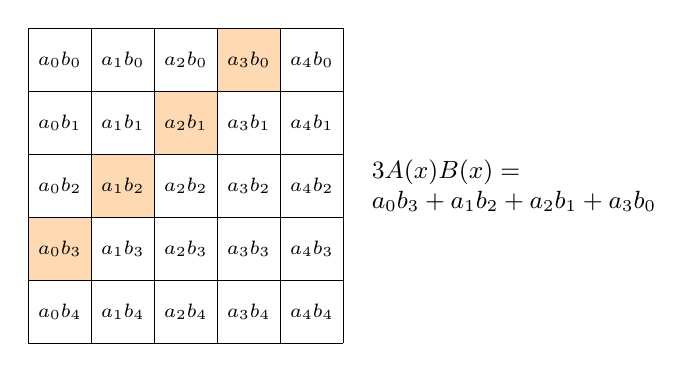
\begin{tikzpicture}[scale=0.8]
  \foreach \i in {0,...,4} { \foreach \j in {0,...,4} {
    \pgfmathtruncatemacro{\s}{\i+\j}
    \ifnum\s=3 \fill[orange!30] (\i,-\j) rectangle (\i+1,-\j-1); \fi
    \node[font=\scriptsize] at (\i+0.5,-\j-0.5) {$a_{\i}b_{\j}$};
  } }
  \draw (0,0) grid (5,-5);
  \node[right,font=\small,align=left] at (5.3,-2.5) {$\coef{3}A(x)B(x) =$\\$a_0b_3 + a_1b_2 + a_2b_1 + a_3b_0$};
\end{tikzpicture}
\end{center}

\begin{lemma}[String lemma]
Let $A$ be a set with weight function $w$ and \emph{no element of weight $0$}. Let
$A^* = \bigcup_{k\ge 0} A^k$ be the set of all finite sequences of elements of $A$ (including the
empty sequence), with the weight of a sequence the sum of the weights of its entries. Then
\[
\Phi_{A^*}(x) = \frac{1}{1 - \Phi_A(x)}.
\]
\end{lemma}
\begin{proof}
The sets $A^k$ are pairwise disjoint, so by the sum and product lemmas
$\Phi_{A^*} = \sum_{k \ge 0} \Phi_A(x)^k$. Since $\Phi_A$ has constant term $0$ this composition
is well defined and equals $1/(1 - \Phi_A(x))$.
\end{proof}

The hypothesis matters: if $A$ had an element of weight $0$ there would be infinitely many
sequences of weight $0$, and $w$ would not be a weight function on $A^*$.

\section{Worked examples}

\begin{example}
How many solutions are there to $a + b = n$ with $a \in \{0,1,2\}$ and $b \ge 0$ even?
The solution set is $\{0,1,2\} \times \{0,2,4,\dots\}$ with weight $a + b$, so
\[
\Phi(x) = (1 + x + x^2)\cdot\frac{1}{1-x^2}
= \sum_{m\ge0} x^{2m} + \sum_{m\ge0}x^{2m+1} + \sum_{m\ge0} x^{2m+2}.
\]
For $n$ odd only the middle sum contributes: $1$ solution. For $n$ even, $n \ge 2$, the first and
third sums each contribute: $2$ solutions; for $n = 0$, $1$ solution. Check $n=4$:
$(0,4), (2,2)$. Correct.
\end{example}

\begin{example}
How many ways can $n$ cents be made from pennies, nickels and dimes (order irrelevant)?
A choice is a triple $(p, k, d)$ of counts with $p + 5k + 10d = n$:
\[
\Phi(x) = \frac{1}{(1-x)(1-x^5)(1-x^{10})}.
\]
For $n = 15$: the possibilities with $d = 0$ are $k \in\{0,1,2,3\}$ ($4$ ways) and with $d = 1$
are $k \in \{0,1\}$ ($2$ ways), so $\coef{15}\Phi = 6$.
\end{example}

\begin{example}
Find $\coef{n} \frac{1 + 2x}{(1-x)^3}$. By the negative binomial theorem,
\[
\coef{n}\frac{1+2x}{(1-x)^3} = \binom{n+2}{2} + 2\binom{n+1}{2}
= \frac{(n+2)(n+1) + 2(n+1)n}{2} = \frac{(n+1)(3n+2)}{2},
\]
valid for all $n \ge 0$ (at $n = 0$ the second term is $\binom{1}{2} = 0$; the formula gives $1$).
\end{example}

\section{Summary}
\begin{itemize}
  \item $\Phi_S(x) = \sum_{\sigma\in S} x^{w(\sigma)}$; $\coef{n}\Phi_S$ counts objects of weight $n$.
  \item Formal power series: add/multiply coefficientwise/by convolution; $A$ invertible iff $a_0\ne0$.
  \item $\frac{1}{1-x} = \sum x^n$, $\frac{1}{(1-x)^k} = \sum \binom{n+k-1}{k-1}x^n$.
  \item Sum lemma (disjoint union), product lemma (Cartesian product, weights add), string lemma
        $\Phi_{A^*} = 1/(1-\Phi_A)$ when $A$ has no weight-$0$ element.
\end{itemize}
